The Qucs-S Attenuator Tool is aimed to synthesize RF attenuators based on the user's input design requirements. Once the synthesis is done, the tool copies a schematic to the clipboard, ready for simulation in Qucs-S. Table \ref{tbl:attenuator-topologies} shows the available topologies.

\begin{center}
  \begin{tabular}{ |l|c|c| }
    \hline
    \textbf{Type} & \textbf{Matched} & \textbf{Broadband} \\ \hline
    $\pi$-type & \checkmark  & \checkmark  \\ \hline
    T-type & \checkmark  & \checkmark  \\ \hline
    Bridged-T & \checkmark  & \checkmark  \\ \hline
    Reflection attenuator & \checkmark  & \checkmark  \\ \hline
    Quarter-wavelength series & $\times$ (1 port only) & $\times$ \\ \hline
    Quarter-wavelength shunt & $\times$ (1 port only) & $\times$ \\ \hline
    L-pad & $\times$ (1 port only) & \checkmark \\ \hline
    Series resistor & $\times$ & \checkmark  \\ \hline
    Shunt resistor & $\times$ & \checkmark  \\ \hline
  \end{tabular}
  \label{tbl:attenuator-topologies}
\end{center}

\noindent As shown in Fig. \ref{fig:qucs-s-attenuator-synthesis-GUI}, the user interface (GUI) has three panels:

\begin{itemize}
	\item \textit{Topology}: It contains a selector to choose among the attenuator topologies in Table \ref{tbl:attenuator-topologies} and a preview image of the circuit topology.
	\item \textit{Input}: This panel contains the input variables for the design such as the attenuation and the input and output impedances. Optionally, the input power can also be specified.
	\item \textit{Output}: It contains the design values to implement the attenuator according to the selected topology. The power dissipated per resistor is also calculated based on the input power data.
\end{itemize}

\noindent Below the topology panel, a checkbox allows the user to automatically include an S-parameter simulation block in the schematic after the synthesis.

  \begin{figure}[ht]
    \centering
    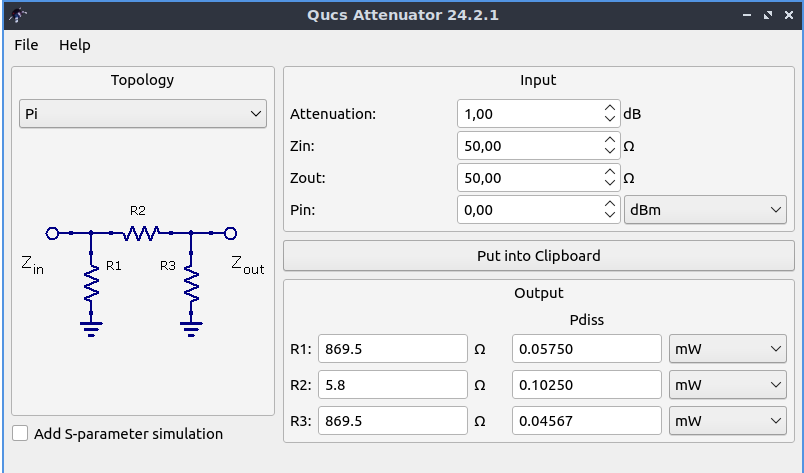
\includegraphics[width=10cm]{./images/Qucs-S-attenuator-synthesis-GUI.png}
    \caption{Qucs-S attenuator synthesis GUI}
    \label{fig:qucs-s-attenuator-synthesis-GUI}
  \end{figure}

\clearpage
\subsubsection{$\pi$-type attenuator}
	\subfile{pi-attenuator}

\clearpage
\subsubsection{T-type attenuator}
	\subfile{tee-attenuator}

\clearpage
\subsubsection{Bridged-T attenuator}
	\subfile{bridged-tee-attenuator}

\clearpage
\subsubsection{Reflection attenuator}
	\subfile{reflection-attenuator}

\clearpage
\subsubsection{Quarter-wavelength series}
	\subfile{qw-series-attenuator}

\clearpage
\subsubsection{Quarter-wavelength shunt}
	\subfile{qw-shunt-attenuator}

\clearpage
\subsubsection{L-pad ($1^{st}$ series)}
	\subfile{L-pad-1st-series-attenuator}

\clearpage
\subsubsection{L-pad ($1^{st}$ shunt)}
	\subfile{L-pad-1st-shunt-attenuator}

\clearpage
\subsubsection{Series resistor}
	\subfile{R-series-attenuator}

\clearpage
\subsubsection{Shunt resistor}
	\subfile{R-shunt-attenuator}
